\documentclass[12pt,a4paper,openany]{book}

% ─── Packages ───────────────────────────────────────────────────────────────
\usepackage[T1]{fontenc}
\usepackage[utf8]{inputenc}
\usepackage{lmodern}
\usepackage[a4paper, top=2.5cm, bottom=2.5cm, left=3cm, right=2.5cm]{geometry}
\usepackage{graphicx}
\usepackage{xcolor}
\usepackage{titlesec}
\usepackage{titletoc}
\usepackage{tocloft}
\usepackage{fancyhdr}
\usepackage{hyperref}
\usepackage{enumitem}
\usepackage{booktabs}
\usepackage{array}
\usepackage{tabularx}
\usepackage{mdframed}
\usepackage{fontawesome5}
\let\faSignInAlt\relax\newcommand{\faSignInAlt}{\faArrowRight}
\let\faShieldAlt\relax\newcommand{\faShieldAlt}{\faExclamationTriangle}
\let\faCheckDouble\relax\newcommand{\faCheckDouble}{\faCheck}
\let\faVoteYea\relax\newcommand{\faVoteYea}{\faThumbsUp}
\usepackage{tikz}
\usetikzlibrary{positioning}
\usepackage{amsmath}
\usepackage{amssymb}
\usepackage{microtype}
\usepackage{setspace}
\usepackage{etoolbox}
\usepackage{parskip}
\usepackage{float}
\usepackage{caption}
\usepackage{subcaption}
\usepackage{multirow}
\usepackage{longtable}
\usepackage{colortbl}
\usepackage{tcolorbox}
\tcbuselibrary{skins,breakable,theorems}

% ─── Colour Palette ──────────────────────────────────────────────────────────
\definecolor{primaryblue}{HTML}{1A3A5C}
\definecolor{accentteal}{HTML}{0D7C8F}
\definecolor{lightgray}{HTML}{F5F7FA}
\definecolor{warningyellow}{HTML}{FFF3CD}
\definecolor{warningborder}{HTML}{FBBF24}
\definecolor{successgreen}{HTML}{D1FAE5}
\definecolor{successborder}{HTML}{10B981}
\definecolor{infoblue}{HTML}{DBEAFE}
\definecolor{infoborder}{HTML}{3B82F6}
\definecolor{dangered}{HTML}{FEE2E2}
\definecolor{dangerborder}{HTML}{EF4444}
\definecolor{sectiongray}{HTML}{6B7280}
\definecolor{coverbg}{HTML}{1E3A5F}

% ─── Hyperref Setup ──────────────────────────────────────────────────────────
\hypersetup{
  colorlinks=true,
  linkcolor=primaryblue,
  urlcolor=accentteal,
  citecolor=accentteal,
  pdftitle={AmarVote -- Voter's Guide},
  pdfauthor={AmarVote},
  pdfsubject={Voter Tutorial},
}

% ─── Custom Boxes ────────────────────────────────────────────────────────────
\tcbset{
  notebox/.style={
    enhanced, breakable,
    colback=infoblue, colframe=infoborder,
    fonttitle=\bfseries\color{primaryblue},
    title={\faInfoCircle\quad Note},
    left=6pt, right=6pt, top=4pt, bottom=4pt,
    arc=4pt
  },
  warnbox/.style={
    enhanced, breakable,
    colback=warningyellow, colframe=warningborder,
    fonttitle=\bfseries\color{orange!80!black},
    title={\faExclamationTriangle\quad Important},
    left=6pt, right=6pt, top=4pt, bottom=4pt,
    arc=4pt
  },
  tipbox/.style={
    enhanced, breakable,
    colback=successgreen, colframe=successborder,
    fonttitle=\bfseries\color{green!50!black},
    title={\faLightbulb\quad Tip},
    left=6pt, right=6pt, top=4pt, bottom=4pt,
    arc=4pt
  },
  dangerbox/.style={
    enhanced, breakable,
    colback=dangered, colframe=dangerborder,
    fonttitle=\bfseries\color{red!70!black},
    title={\faTimesCircle\quad Warning},
    left=6pt, right=6pt, top=4pt, bottom=4pt,
    arc=4pt
  },
  stepbox/.style={
    enhanced, breakable,
    colback=lightgray, colframe=primaryblue,
    fonttitle=\bfseries\color{white},
    attach boxed title to top left={xshift=10pt, yshift=-\tcboxedtitleheight/2},
    boxed title style={colback=primaryblue, arc=3pt},
    left=6pt, right=6pt, top=12pt, bottom=4pt,
    arc=4pt
  },
  conceptbox/.style={
    enhanced, breakable,
    colback=lightgray, colframe=sectiongray,
    fonttitle=\bfseries\color{primaryblue},
    title={\faBook\quad How This Works},
    left=6pt, right=6pt, top=4pt, bottom=4pt,
    arc=4pt
  }
}

% ─── Section Formatting ──────────────────────────────────────────────────────
\titleformat{\chapter}[display]
  {\normalfont\huge\bfseries\color{primaryblue}}
  {\chaptertitlename\ \thechapter}{12pt}{\Huge}
\titlespacing{\chapter}{0pt}{-10pt}{20pt}

\titleformat{\section}
  {\normalfont\Large\bfseries\color{primaryblue}}
  {\thesection}{1em}{}
\titleformat{\subsection}
  {\normalfont\large\bfseries\color{accentteal}}
  {\thesubsection}{1em}{}
\titleformat{\subsubsection}
  {\normalfont\normalsize\bfseries\color{sectiongray}}
  {\thesubsubsection}{1em}{}

% ─── Header / Footer ─────────────────────────────────────────────────────────
\pagestyle{fancy}
\fancyhf{}
\fancyhead[LE,RO]{\small\thepage}
\fancyhead[LO]{\small\nouppercase{\rightmark}}
\fancyhead[RE]{\small\nouppercase{\leftmark}}
\fancyfoot[C]{\small\color{sectiongray}AmarVote --- Voter's Guide}
\renewcommand{\headrulewidth}{0.4pt}

% ─── Custom Commands ─────────────────────────────────────────────────────────
\newcommand{\uibutton}[1]{\colorbox{primaryblue}{\textcolor{white}{\small\textbf{#1}}}}
\newcommand{\uifield}[1]{\texttt{\color{accentteal}#1}}
\newcommand{\uimenu}[1]{\textbf{\color{primaryblue}#1}}
\newcommand{\placeholder}[1]{\textit{\color{sectiongray}[#1]}}

% ─── Figure Helper ───────────────────────────────────────────────────────────
\newcommand{\screenfig}[3][0.92]{%
  \begin{figure}[H]
    \centering
    \includegraphics[width=#1\linewidth]{figures/#2}
    \caption{#3}
    \label{fig:#2}
  \end{figure}%
}

% ─── List Styling ────────────────────────────────────────────────────────────
\setlist[itemize,1]{label=\textcolor{accentteal}{\faChevronRight}, leftmargin=1.5em}
\setlist[itemize,2]{label=\textcolor{sectiongray}{\faCircle[regular]}, leftmargin=2em}
\setlist[enumerate,1]{label=\textcolor{primaryblue}{\textbf{\arabic*.}}, leftmargin=2em}

\setstretch{1.15}

% ════════════════════════════════════════════════════════════════════════════
\begin{document}

% ─── COVER PAGE ──────────────────────────────────────────────────────────────
\begin{titlepage}
	\pagecolor{coverbg}
	\color{white}
	\centering
	\vspace*{2cm}

	{\fontsize{60}{65}\selectfont\bfseries AmarVote}

	\vspace{0.5cm}
	{\Large\color{accentteal} Secure Cryptographic Voting Platform}

	\vspace{1.5cm}
	\hrule width 12cm height 0.5pt
	\vspace{0.4cm}
	{\LARGE\bfseries Voter's Guide}
	\vspace{0.2cm}
	{\large\color{accentteal} A Complete Step-by-Step Tutorial for Voters}
	\vspace{0.4cm}
	\hrule width 12cm height 0.5pt

	\vspace{2cm}

	\begin{tcolorbox}[
			enhanced, width=10cm,
			colback=primaryblue!80!black, colframe=accentteal,
			arc=6pt, boxrule=1.5pt,
			left=12pt, right=12pt, top=10pt, bottom=10pt
		]
		\centering\color{white}
		\textbf{This guide covers everything a voter needs to know:}\\[6pt]
		\textcolor{accentteal}{\faUserPlus} \, Registering Your Account\\[4pt]
		\textcolor{accentteal}{\faSignInAlt} \, Logging In Securely\\[4pt]
		\textcolor{accentteal}{\faShieldAlt} \, Setting Up Two-Factor Authentication\\[4pt]
		\textcolor{accentteal}{\faVoteYea} \, Finding an Election \& Entering the Voting Booth\\[4pt]
		\textcolor{accentteal}{\faLock} \, Creating Your Encrypted Ballot\\[4pt]
		\textcolor{accentteal}{\faQuestion} \, Performing the Benaloh Challenge\\[4pt]
		\textcolor{accentteal}{\faPaperPlane} \, Casting Your Vote \& Receiving Your Receipt\\[4pt]
		\textcolor{accentteal}{\faCheckDouble} \, Verifying Your Ballot After Results Are Published
	\end{tcolorbox}

	\vfill

	\begin{tabular}{cc}
		\textcolor{accentteal}{\faLock} \, ElectionGuard Powered &
		\textcolor{accentteal}{\faEye} \, End-to-End Verifiable
	\end{tabular}

	\vspace{1cm}
	{\small Version 1.0 \quad|\quad \today}
\end{titlepage}
\nopagecolor
\color{black}

% ─── FRONT MATTER ────────────────────────────────────────────────────────────
\frontmatter
\tableofcontents

\chapter*{Welcome to AmarVote}
\addcontentsline{toc}{chapter}{Welcome to AmarVote}

This guide is written \textbf{specifically for you --- a voter}. You do not need any technical background. You do not need to understand cryptography. You only need to follow the steps in this guide, and AmarVote will take care of the rest.

AmarVote is a secure online voting platform built on a technology called \textbf{ElectionGuard}. In plain language, this means:

\begin{itemize}
	\item \textbf{Your vote is encrypted before it is stored at the database} It is never stored in plaintext. Not even the election administrator or AmarVote staff can see how you voted.
	\item \textbf{You receive a receipt.} After you vote, you get an email with a tracking code that proves your ballot was recorded.
	\item \textbf{You can verify your vote yourself.} After the election results are published, you can upload your receipt and the system will confirm your ballot was counted --- without anyone ever knowing how you voted.
\end{itemize}

\begin{tcolorbox}[tipbox]
	Read this guide from start to finish the first time. After that, use the Table of Contents to jump quickly to any step you need to revisit.
\end{tcolorbox}

\section*{Your Journey at a Glance}

\begin{center}
	\begin{tikzpicture}[
		node distance=0.6cm,
		box/.style={draw, rounded corners, fill=infoblue, text width=3.2cm, align=center,
			font=\small, minimum height=1.1cm, inner sep=4pt},
		arrow/.style={->, thick, color=accentteal}
	]
		\node[box] (A) {\faUserPlus\\[2pt]\textbf{Register}};
		\node[box, right=of A] (B) {\faSignInAlt\\[2pt]\textbf{Log In}};
		\node[box, right=of B] (C) {\faShieldAlt\\[2pt]\textbf{Enable 2FA}};
		\node[box, right=of C] (D) {\faSearch\\[2pt]\textbf{Find Election}};
		\node[box, below=1.2cm of D] (E) {\faLock\\[2pt]\textbf{Encrypt \& Cast}};
		\node[box, left=of E] (F) {\faPaperPlane\\[2pt]\textbf{Receive Receipt}};
		\node[box, left=of F] (G) {\faCheckDouble\\[2pt]\textbf{Verify Ballot}};
		\draw[arrow] (A)--(B);
		\draw[arrow] (B)--(C);
		\draw[arrow] (C)--(D);
		\draw[arrow] (D)--(E);
		\draw[arrow] (E)--(F);
		\draw[arrow] (F)--(G);
	\end{tikzpicture}
\end{center}

% ════════════════════════════════════════════════════════════════════════════
\mainmatter

% ════════════════════════════════════════════════════════════════════════════
\chapter{Creating Your Account}
\label{ch:registration}

Before you can vote on AmarVote, you need to create a personal account. The process is quick and takes only a few minutes. You will verify your email address and set a password --- nothing more is required at this stage.

\begin{tcolorbox}[warnbox]
	\textbf{Prerequisite:} You can only register if your email address has already been added to AmarVote's Authorised User List by the platform administrator. If you try to register with an email that is not on the list, the system will reject it. If this happens, contact the person who invited you to the election.
\end{tcolorbox}

\section{Overview of the Registration Steps}

The full registration process follows this sequence:

\begin{center}
	\textbf{Home Page} \;\faArrowRight\; \textbf{Click Register} \;\faArrowRight\; \textbf{Enter Your Email} \;\faArrowRight\; \textbf{Receive Verification Code} \;\faArrowRight\; \textbf{Enter the Code} \;\faArrowRight\; \textbf{Set a Password} \;\faArrowRight\; \textbf{Account Ready}
\end{center}

\section{Step 1 --- Open AmarVote and Go to the Registration Page}

\begin{enumerate}
	\item Open your web browser (Chrome, Firefox, Edge, Safari --- any modern browser works).
	\item Navigate to the AmarVote URL provided by your organisation.
	\item You will see the \textbf{AmarVote home page}.

	      \screenfig{homeAmarVote.png}{The AmarVote home page --- your starting point}

	\item Click the \uibutton{Register} button. This takes you to the registration form.
\end{enumerate}

\section{Step 2 --- Enter Your Email Address}

\begin{enumerate}
	\item The registration page will display a field asking for your email address.

	      \screenfig{verifyEmailForRegistering.png}{The registration form --- enter your email address here}

	\item Type the email address that was added to the Authorised User List. This must be an \textbf{exact match} --- even a small difference (such as a dot or a capital letter) will cause a rejection.
	\item Click \uibutton{Send Verification Code}.
	\item AmarVote will send a \textbf{6-digit One-Time Password (OTP)} to that email address. A confirmation screen will appear telling you the code has been sent.

	      \screenfig{codeSentToEmail.png}{The confirmation screen after requesting your verification code}
\end{enumerate}

\begin{tcolorbox}[tipbox]
	Check your \textbf{spam} or \textbf{junk} folder if you do not receive the email within two minutes. The code is valid for \textbf{10 minutes}. If it expires before you enter it, go back to the registration page and request a new one.
\end{tcolorbox}

\section{Step 3 --- Enter the Verification Code}

\begin{enumerate}
	\item Open the email from AmarVote and find the \textbf{6-digit verification code}.
	\item Go back to the AmarVote registration page in your browser (it should still be open).
	\item Type the 6-digit code into the \uifield{Verification Code} field.

	      \screenfig{enterTheVerificationCode.png}{Entering the 6-digit code to verify your email address}

	\item Click \uibutton{Verify Email}.
	\item If the code is correct and has not expired, the page will automatically advance to the next step.
\end{enumerate}

\begin{tcolorbox}[notebox]
	Each verification code can only be used once. Once you enter it successfully, it is invalidated. If you accidentally enter it twice or use an expired code, simply request a fresh one.
\end{tcolorbox}

\section{Step 4 --- Set Your Password}

\begin{enumerate}
	\item The password creation screen will now appear.

	      \screenfig{setYourPassword.png}{The password setup screen --- choose a strong password}

	\item Enter a \textbf{strong password} in the \uifield{Password} field. A strong password should be:
	      \begin{itemize}
		      \item At least \textbf{8 characters} long.
		      \item A mix of \textbf{uppercase letters, lowercase letters, numbers}, and \textbf{symbols} (e.g., \texttt{@}, \texttt{\#}, \texttt{!}).
		      \item Something \textbf{unique} that you do not use on other websites.
	      \end{itemize}
	\item Re-enter the exact same password in the \uifield{Confirm Password} field.
	\item Click \uibutton{Create Account}.
	\item Your account will be created and you will be redirected to the login page.
\end{enumerate}

\begin{tcolorbox}[dangerbox]
	\textbf{Never share your password.} AmarVote staff and election administrators will \emph{never} ask for your password. If anyone asks you for it, refuse. Consider storing your password in a trusted password manager such as Bitwarden, 1Password, or your browser's built-in password vault.
\end{tcolorbox}

% ════════════════════════════════════════════════════════════════════════════
\chapter{Logging In to AmarVote}
\label{ch:login}

Once you have a registered account, logging in is simple. You will use the same email and password you set during registration.

\section{Overview of the Login Steps}

\begin{center}
	\textbf{Home Page} \;\faArrowRight\; \textbf{Click Login} \;\faArrowRight\; \textbf{Enter Email \& Password} \;\faArrowRight\; \textbf{Dashboard}
\end{center}

If you have Two-Factor Authentication enabled (recommended and explained in the next chapter), there is one additional step:

\begin{center}
	\textbf{Home Page} \;\faArrowRight\; \textbf{Click Login} \;\faArrowRight\; \textbf{Enter Email \& Password} \;\faArrowRight\; \textbf{Enter 2FA Code} \;\faArrowRight\; \textbf{Dashboard}
\end{center}

\section{Standard Login}

\begin{enumerate}
	\item Open your web browser and navigate to the AmarVote URL.
	\item On the home page, click \uibutton{Login}.

	      \screenfig{homeAmarVote.png}{The AmarVote home page --- click \textit{Login} to begin}

	\item The login screen will appear.

	      \screenfig{loginScreen.png}{The AmarVote login screen --- enter your email and password}

	\item Enter your registered \uifield{Email Address}.
	\item Enter your \uifield{Password}.
	\item Click \uibutton{Continue}.
	\item You will be taken to your \textbf{Dashboard} --- the main page you see after every login.
\end{enumerate}

\section{Login with Two-Factor Authentication}

If you have enabled 2FA (see Chapter~\ref{ch:2fa}), after you enter your email and password and click \uibutton{Continue}, one extra step appears:

\begin{enumerate}
	\item A prompt will ask you for your \uifield{Authenticator Code}.
	\item Open the Google Authenticator (or Authy, or Microsoft Authenticator) app on your smartphone.
	\item Find the \textbf{AmarVote entry} in the app. A rotating 6-digit code will be displayed.
	\item Type this code into the prompt and click \uibutton{Verify}.
	\item You will be taken to your Dashboard.
\end{enumerate}

\begin{tcolorbox}[notebox]
	The code in your authenticator app changes every \textbf{30 seconds}. If the code expires while you are typing, simply wait for the next code to appear and use that one instead.
\end{tcolorbox}

\section{Forgot Your Password?}

If you cannot remember your password:

\begin{enumerate}
	\item On the login screen, click \uimenu{Forgot Password?}.
	\item Enter your registered \uifield{Email Address} and click \uibutton{Send Verification Code}.
	\item Check your inbox for a password reset code (check spam if it does not arrive quickly).
	\item Enter the code on the reset page, then choose and confirm a new password.
	\item Log in immediately with your new password.
\end{enumerate}

% ════════════════════════════════════════════════════════════════════════════
\chapter{Setting Up Two-Factor Authentication (2FA)}
\label{ch:2fa}

Two-Factor Authentication (2FA) adds a vital second layer of security to your account. Even if someone discovers your password, they still cannot log in without the unique code from your personal smartphone.

\begin{tcolorbox}[warnbox]
	\textbf{2FA is strongly recommended for all voters.} Elections involve sensitive decisions. Protecting your account with 2FA ensures that only you can cast your vote.
\end{tcolorbox}

\begin{tcolorbox}[conceptbox]
	\textbf{What is 2FA?}

	Normally, logging in requires just one thing you know: your password. Two-Factor Authentication adds a second requirement --- something you \emph{have}: your smartphone. The authenticator app on your phone generates a new 6-digit code every 30 seconds using a secret key shared only between your phone and AmarVote. Even if someone steals your password, they cannot log in without also holding your physical phone.
\end{tcolorbox}

\section{What You Need}

Before you begin, install one of these free authenticator apps on your smartphone:

\begin{itemize}
	\item \textbf{Google Authenticator} --- Available on iOS (App Store) and Android (Google Play)
	\item \textbf{Microsoft Authenticator} --- Available on iOS and Android
	\item \textbf{Authy} --- Available on iOS, Android, and desktop (also supports cloud backup)
\end{itemize}

\section{How to Enable 2FA}

\begin{enumerate}
	\item Log in to your AmarVote account.
	\item In the top-right corner of the screen, click your \textbf{profile avatar} (your initials or photo).

	      \screenfig{goToProfileMenu.png}{Clicking the profile avatar to access account settings}

	\item A dropdown menu will appear. Click \uibutton{Enable Two-Factor Authentication}.
	\item The 2FA setup screen will appear, displaying a \textbf{QR code}.

	      \screenfig{enable2FactorAuthentication.png}{The 2FA setup screen with the QR code to scan}

	\item Open your authenticator app on your smartphone.
	\item Tap the \textbf{+} button (or ``Add Account'') and select \uimenu{Scan a QR code}.
	\item Point your phone's camera at the QR code on your screen. The app will automatically register AmarVote.
	\item Your app will now show a rotating 6-digit code labelled ``AmarVote'' (or similar).
	\item Type the current 6-digit code from your app into the \uifield{Verification Code} field on AmarVote.
	\item Click \uibutton{Confirm}. 2FA is now active on your account.
\end{enumerate}

\begin{tcolorbox}[dangerbox]
	\textbf{Do not lose access to your authenticator app.} If you lose or replace your phone without transferring your authenticator accounts, you may be permanently locked out of AmarVote. If you use Authy, enable its encrypted cloud backup feature. For Google Authenticator, enable Google Account sync (available in the app settings).
\end{tcolorbox}

% ════════════════════════════════════════════════════════════════════════════
\chapter{Finding Your Election}
\label{ch:finding}

After logging in, you need to locate the election you want to vote in. There are two ways to do this: through your \textbf{Dashboard} or through the \textbf{All Elections} page.

\section{Method 1 --- From Your Dashboard}

When you log in, your Dashboard shows a summary of ongoing and upcoming elections you are eligible to vote in. If the election is currently active, it may appear directly on your Dashboard as a card or notification.

\screenfig{findCurrentElectionsInDashboard.png}{Active elections may appear directly on your Dashboard after logging in}

\begin{enumerate}
	\item After logging in, look for an election card on your Dashboard.
	\item Click on the election's name or card to open the election page.
\end{enumerate}

\section{Method 2 --- From the All Elections Page}

If the election does not appear on your Dashboard, or if you want to browse all available elections:

\begin{enumerate}
	\item Click the \textbf{menu icon} at the top of the left-side navigation sidebar to open the navigation menu.

	      \screenfig{openMenu.png}{Opening the navigation menu from the sidebar}

	\item Click \uimenu{All Elections} in the menu.

	      \screenfig{menuSelectAllElections.png}{Selecting \textit{All Elections} from the navigation menu}

	\item The All Elections page will show a list of elections. Use the \uimenu{Ongoing} filter tab to display only elections that are currently open for voting.

	      \screenfig{findCurrentElectionsInAllElectionsSelectingOngoingOption.png}{Using the \textit{Ongoing} filter to find currently active elections}

	\item Find the election you want to participate in and click its name to open the election page.
\end{enumerate}

\begin{tcolorbox}[notebox]
	You will only be able to vote in elections where:
	\begin{itemize}
		\item The election is currently \textbf{open} (it has started and not yet ended).
		\item Your email is on the election's approved voter list, \emph{or} the election is open to all registered users.
		\item You have \textbf{not} already cast your final vote in this election.
	\end{itemize}
	If none of these conditions are met, the Voting Booth will not be available to you.
\end{tcolorbox}

% ════════════════════════════════════════════════════════════════════════════
\chapter{Inside the Voting Booth}
\label{ch:voting}

This is the main event. The Voting Booth is where you make your selection, create your encrypted ballot, verify it with the Benaloh Challenge, and finally cast your vote. Each of these steps is explained carefully below.

\begin{tcolorbox}[conceptbox]
	\textbf{Why is there so many steps instead of just clicking a candidate and being done?}

	AmarVote uses a system called \textbf{end-to-end verifiable voting}. This means the system is designed so that anyone --- including you --- can mathematically confirm the election is honest, without requiring you to simply \emph{trust} the software. The extra steps (encryption, Benaloh Challenge, receipt) are what make this guarantee possible. They take less than two minutes once you understand them.
\end{tcolorbox}

\section{Accessing the Voting Booth}

\begin{enumerate}
	\item Open the election page (see Chapter~\ref{ch:finding}).
	\item On the election page, click the \uimenu{Voting Booth} tab.

	      \screenfig{votingBoothShowingEligibility.png}{The Voting Booth tab showing your eligibility to vote}
\end{enumerate}

\begin{tcolorbox}[warnbox]
	The \uimenu{Voting Booth} tab only appears if:
	\begin{itemize}
		\item The election is currently open.
		\item You are on the approved voter list (or the election is open to all users).
		\item You have not already cast your final ballot.
	\end{itemize}
	If you do not see the tab, one of these conditions is not met. Check that the election is still within its voting period and that you are using the correct account.
\end{tcolorbox}

\section{Step 1 --- Select Your Candidate(s)}

\begin{enumerate}
	\item Inside the Voting Booth, you will see all candidates listed with their names and photos (if the election administrator uploaded photos).
	\item The ballot will tell you how many candidates you may choose, for example: \emph{``Select up to 1 candidate''} or \emph{``Select up to 2 candidates.''} Follow this instruction.
	\item Click on the candidate(s) you want to vote for. A checkmark will appear next to each selected candidate.
	\item When you are ready, click \uibutton{Create Encrypted Ballot}.
\end{enumerate}

\screenfig{createEncryptedBallot.png}{Selecting your candidate(s) inside the Voting Booth}

\begin{tcolorbox}[notebox]
	\textbf{Clicking ``Create Encrypted Ballot'' does NOT cast your vote.} This step only prepares a secure, encrypted version of your choice. You still need to decide whether to \textbf{verify} it (Benaloh Challenge) or \textbf{cast} it. Both options are explained next.
\end{tcolorbox}

\screenfig{encryptedBallotCreatedSuccessfully.png}{Confirmation that your encrypted ballot has been successfully created}

After clicking \uibutton{Create Encrypted Ballot}, a confirmation message appears. Your ballot is now encrypted. You will see two buttons:
\begin{itemize}
	\item \uibutton{Challenge Ballot (Benaloh Challenge)} --- to verify the encryption is correct.
	\item \uibutton{Cast Ballot} --- to submit your vote permanently.
\end{itemize}

Both options are fully explained in the sections that follow.

% ════════════════════════════════════════════════════════════════════════════
\chapter{The Benaloh Challenge --- Verifying Your Encryption}
\label{ch:benaloh}

The \textbf{Benaloh Challenge} is an optional but highly recommended step. It lets you confirm that the system actually encrypted what you selected --- and not something else. You can run this check as many times as you wish before you cast your final vote.

\section{Why Does This Exist?}

\begin{tcolorbox}[conceptbox]
	\textbf{The problem the Benaloh Challenge solves:}

	When your vote is encrypted, it becomes a block of scrambled data that is unreadable. How do you know the software encrypted your \emph{actual} choice, and not a different candidate? You can't just decrypt it to check, because that would reveal how you voted to the server.

	The Benaloh Challenge solves this cleverly. When you challenge a ballot, the system reveals the \emph{internal random numbers} used to create that specific encryption. You then re-enter what you intended to vote for, and the system checks whether those random numbers and your stated choice produce the \emph{same} encrypted result. If they do, the encryption is verified correct. If they do not, the system has made an error (which should never happen in a properly functioning implementation).

	\textbf{The key insight:} Because the system must reveal the random numbers to you, it cannot cheat. If it encrypted the wrong thing, the revealed numbers would not match --- and the challenge would fail.

	The challenged ballot is always discarded and never counted, so performing the challenge is completely safe.
\end{tcolorbox}

\section{How to Perform the Benaloh Challenge}

After you click \uibutton{Create Encrypted Ballot} and see the confirmation message:

\begin{enumerate}
	\item Click \uibutton{Challenge Ballot (Benaloh Challenge)}.
	\item A selection interface will appear --- the same interface where you chose your candidates. This time, you are being asked: \emph{``What did you intend to vote for?''}
	\item Select the same candidate(s) you originally chose.

	      \screenfig{benalohChallengeCorrectSelection.png}{The Benaloh Challenge interface --- re-select the same candidates you originally chose}

	\item Click \uibutton{Submit Challenge}.
	\item The system will check whether your stated choice matches the encrypted ballot.
\end{enumerate}

\section{Understanding the Result}

\begin{figure}[H]
	\centering
	\begin{subfigure}[b]{0.48\textwidth}
		\centering
		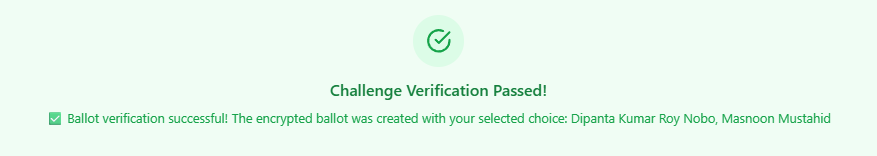
\includegraphics[width=\textwidth]{figures/benalohChallengePassed.png}
		\caption{Challenge passed --- the encryption is verified correct}
		\label{fig:benaloh-passed}
	\end{subfigure}
	\hfill
	\begin{subfigure}[b]{0.48\textwidth}
		\centering
		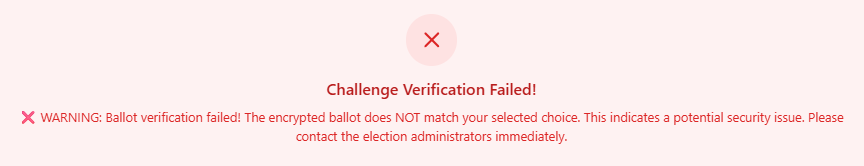
\includegraphics[width=\textwidth]{figures/benalohChallengeFailed.png}
		\caption{Challenge failed --- this indicates an encryption mismatch}
		\label{fig:benaloh-failed}
	\end{subfigure}
	\caption{Benaloh Challenge outcomes: passed (left) and failed (right)}
	\label{fig:benaloh-outcomes}
\end{figure}

\begin{itemize}
	\item \textbf{Challenge Passed} --- The encryption was correct. The system encrypted exactly what you selected. You can now proceed to cast your vote with confidence.
	\item \textbf{Challenge Failed} --- The re-entered selection did not match the encrypted ballot. This will happen if you selected a \emph{different} set of candidates in the challenge than you originally voted for. For example, if you voted for Candidate A, but entered Candidate B during the challenge, the challenge will fail --- which is the correct and expected behaviour. It is not an error; it is the system working as intended.
\end{itemize}

\screenfig{benalohChallengeIncorrectSelection.png}{Example of an incorrect candidate selection causing the Benaloh Challenge to fail}

\begin{tcolorbox}[dangerbox]
	\textbf{The challenged ballot is permanently discarded.} Whether the challenge passes or fails, the encrypted ballot you just challenged \textbf{will never be counted}. This is by design --- it ensures that anyone could challenge a ballot without fear of it becoming their final vote.

	After a challenge, you must:
	\begin{enumerate}
		\item Go back to the Voting Booth.
		\item Re-select your candidate(s).
		\item Click \uibutton{Create Encrypted Ballot} again.
		\item Then decide to challenge again or cast your vote.
	\end{enumerate}
\end{tcolorbox}

\begin{tcolorbox}[tipbox]
	\textbf{You may challenge as many times as you like.} There is no limit. Each challenge creates a new encrypted ballot, which you may challenge again or cast. Feel free to run the challenge multiple times to build confidence in the system --- just remember that you must eventually \emph{cast} (not challenge) a ballot for your vote to be counted.
\end{tcolorbox}

% ════════════════════════════════════════════════════════════════════════════
\chapter{Casting Your Vote}
\label{ch:casting}

When you are satisfied that the system is working correctly and are ready to submit your final vote:

\section{How to Cast Your Ballot}

\begin{enumerate}
	\item If you have just performed a Benaloh Challenge, go back to the Voting Booth and re-select your candidate(s).
	\item If you are continuing from a freshly created encrypted ballot (without challenging), you are already at this step.
	\item You will see two buttons: \uibutton{Challenge Ballot (Benaloh Challenge)} and \uibutton{Cast Ballot}.
	\item Click \uibutton{Cast Ballot}.
\end{enumerate}

\screenfig{castEncryptedBallot.png}{Clicking \textit{Cast Ballot} to submit your vote permanently}

\begin{tcolorbox}[dangerbox]
	\textbf{This action is permanent and irreversible.} Once you click \uibutton{Cast Ballot}, your vote is submitted to the system and \textbf{cannot be changed, recalled, or re-cast}. Make absolutely sure you have selected the right candidate(s) before casting.
\end{tcolorbox}

After casting, the system will confirm that your vote has been recorded. If you attempt to vote again, the system will prevent you:

\screenfig{cantVoteMultipleTimes.png}{The system prevents a voter from casting more than one ballot}

\section{Your Voter Receipt Email}

Within a short time of casting your ballot, AmarVote will automatically send you an email containing your \textbf{Voter Receipt}. This email is very important --- \textbf{do not delete it}.

\screenfig{ballotReceiptReceivedByEmailAfterCastingVote.png}{The voter receipt email received after successfully casting your encrypted ballot}

Your receipt contains two key pieces of information:

\begin{center}
	\begin{tabularx}{0.9\textwidth}{>{\bfseries}l X}
		\toprule
		\rowcolor{primaryblue}\color{white}Item & \color{white}What It Is\\
		\midrule
		\rowcolor{lightgray}Ballot Tracking Code & A unique identifier for your ballot in the public tally. Used to find your ballot after results are published.\\
		Ballot Hash & A cryptographic fingerprint of your encrypted ballot. Used to confirm your ballot was not modified after submission.\\
		\bottomrule
	\end{tabularx}
\end{center}

\begin{tcolorbox}[warnbox]
	\textbf{Save your receipt!} You will need this email to verify your vote after the results are published. If you lose it, you will not be able to verify whether your ballot was included in the tally. Keep the email in a safe folder, or copy the Tracking Code and Hash to a secure document.
\end{tcolorbox}

\begin{tcolorbox}[notebox]
	\textbf{Your privacy is protected.} The Ballot Tracking Code and Ballot Hash identify your \emph{ballot} --- not you as a person. The public tally shows these codes but \emph{not} your name, so your identity is never exposed. However, as a best practice, do not share your receipt with others, as it could be used to locate your encrypted ballot in the public tally (though it would still be encrypted and unreadable).
\end{tcolorbox}

% ════════════════════════════════════════════════════════════════════════════
\chapter{Verifying Your Ballot After Results Are Published}
\label{ch:verification}

The election results will be published after the election has closed and the administrators have completed the tallying process. Once published, you can use your voter receipt to independently confirm that your ballot was actually included in the final count.

This is the final step of AmarVote's \textbf{end-to-end verification} promise: \emph{your ballot was cast as intended, recorded as cast, and counted as recorded.}

\begin{tcolorbox}[conceptbox]
	\textbf{What does verification actually prove?}

	When you upload your receipt and the system returns a positive result, two things are confirmed:
	\begin{enumerate}
		\item \textbf{Ballot Found:} Your Ballot Tracking Code exists in the list of ballots that were tallied. This means your ballot was not silently discarded.
		\item \textbf{Hash Match:} The Ballot Hash in the tally matches the Hash in your receipt email. This means your encrypted ballot was not modified or replaced after you submitted it.
	\end{enumerate}
	Together, these two checks confirm that your vote was \emph{counted exactly as you cast it} --- without anyone knowing what candidate you chose.
\end{tcolorbox}

\section{Step 1 --- Wait for Results to Be Published}

Results are published after:
\begin{enumerate}
	\item The election closes (the end time passes).
	\item The election administrators complete the tallying and decryption process (this may take some time after the election ends --- check the election page for status updates).
\end{enumerate}

When results are ready, the election page will display them. You can then proceed to verification.

\section{Step 2 --- Navigate to the ``Verify Your Vote'' Tab}

\begin{enumerate}
	\item Log in to AmarVote.
	\item Navigate to the election page (see Chapter~\ref{ch:finding}).
	\item On the election page, click the \uimenu{Verify Your Vote} tab.
\end{enumerate}

\section{Step 3 --- Upload Your Ballot Receipt}

\begin{enumerate}
	\item On the \uimenu{Verify Your Vote} tab, you will see an upload area.
	\item Click \uibutton{Upload} and select the ballot receipt file you received by email after casting your vote.

	      \screenfig{uploadYouBallotReceiptToVerify.png}{Uploading your ballot receipt file on the Verify Your Vote tab}

	\item The system will process the file and display the result.
\end{enumerate}

\begin{tcolorbox}[tipbox]
	The receipt file is attached to the email you received after voting. It is typically a small \texttt{.json} or similar file. Save it to your device before attempting this step. If you cannot find the attachment, check the email again --- the tracking code and hash may also be in the email body, which you can use for manual verification (see Section~\ref{sec:manual}).
\end{tcolorbox}

\section{Step 4 --- Read the Verification Result}

\screenfig{ballotVerifiedSuccessfully.png}{Successful verification --- the system confirms your ballot was recorded and unmodified}

If everything is correct, you will see a \textbf{successful verification message} confirming:
\begin{itemize}
	\item \faCheckCircle\ \textcolor{successborder}{\textbf{Ballot Found}} --- Your tracking code was found in the tally.
	\item \faCheckCircle\ \textcolor{successborder}{\textbf{Hash Match}} --- Your ballot was not altered after you submitted it.
\end{itemize}

This means your vote was counted exactly as you cast it. Congratulations --- you have completed the full end-to-end verification process.

\begin{tcolorbox}[dangerbox]
	\textbf{What if the hash does not match?} If the system reports a hash mismatch, this is a serious indication that your ballot may have been tampered with after submission. Report this immediately to the Election Administrator and your relevant institutional or national election authority. Do not discard your receipt email --- preserve it as evidence.
\end{tcolorbox}

\section{Alternative: Manual Ballot Lookup}
\label{sec:manual}

If you prefer to verify your ballot manually without using the upload tool --- or if you want an additional layer of confirmation --- you can also look up your ballot directly in the public tally list:

\begin{enumerate}
	\item On the election page, click the \uimenu{Ballots in Tally} tab.
	\item This tab displays the complete list of all encrypted ballots that were included in the final tally.

	      \screenfig{electionResultsballotsInTally.png}{The \textit{Ballots in Tally} tab showing all ballots included in the tally}

	\item Scroll through the list (or use your browser's \textbf{Ctrl+F} / \textbf{Cmd+F} search function) to find your \textbf{Ballot Tracking Code} from your receipt email.
	\item Once found, compare the \textbf{Ballot Hash} displayed in the tally with the Hash in your receipt email. They should be identical, character for character.
\end{enumerate}

\screenfig{seeIndividualEncryptedBallotContent.png}{Viewing the details of an individual encrypted ballot in the Ballots in Tally list}

\begin{tcolorbox}[notebox]
	The Ballots in Tally list is deliberately public and visible to everyone --- including people who did not vote. This is a feature, not a flaw. It allows anyone to independently audit the election. Ballot tracking codes identify the \emph{ballot}, not the \emph{voter}, so your identity is never exposed in this list.
\end{tcolorbox}

% ════════════════════════════════════════════════════════════════════════════
\chapter{Your Complete Voter Journey --- A Quick Reference}
\label{ch:summary}

Use this chapter as a quick reference card to remind yourself of every step.

\section{Before the Election}

\begin{enumerate}
	\item \textbf{Register} --- Go to the AmarVote URL, click \uibutton{Register}, verify your email with the OTP code, and set a strong password.
	\item \textbf{Enable 2FA} --- After logging in, click your profile avatar, click \uibutton{Enable Two-Factor Authentication}, scan the QR code with your authenticator app, and confirm.
\end{enumerate}

\section{During the Election}

\begin{enumerate}
	\item \textbf{Log In} --- Go to the AmarVote URL, click \uibutton{Login}, enter your email and password (and 2FA code if enabled).
	\item \textbf{Find the Election} --- Check your Dashboard or go to \uimenu{All Elections} and use the \uimenu{Ongoing} filter.
	\item \textbf{Enter the Voting Booth} --- Open the election page and click the \uimenu{Voting Booth} tab.
	\item \textbf{Select Your Candidate(s)} --- Click your choice(s) and click \uibutton{Create Encrypted Ballot}.
	\item \textbf{Optionally Verify (Benaloh Challenge)} --- Click \uibutton{Challenge Ballot}, re-select the same candidate(s), click \uibutton{Submit Challenge}, and check the result. The challenged ballot is discarded. Repeat steps 4--5 as many times as you like.
	\item \textbf{Cast Your Vote} --- When ready, click \uibutton{Cast Ballot}. This is permanent and irreversible.
	\item \textbf{Save Your Receipt} --- Check your email for the Voter Receipt containing your Ballot Tracking Code and Ballot Hash. Do not delete this email.
\end{enumerate}

\section{After the Election (Once Results Are Published)}

\begin{enumerate}
	\item \textbf{Log In} and navigate to the election page.
	\item \textbf{Click ``Verify Your Vote''} and upload your receipt file from your email.
	\item \textbf{Check the result} --- confirm that your ballot was found and the hash matches.
	\item Alternatively, browse the \uimenu{Ballots in Tally} tab and manually search for your Tracking Code.
\end{enumerate}

% ════════════════════════════════════════════════════════════════════════════
\appendix

\chapter{Frequently Asked Questions for Voters}

\section*{Can anyone see how I voted?}

No. Your vote is encrypted before it is stored in the database. The database only stores receives an encrypted block of data --- it never stores your actual choice in plaintext.  Only the final tally is ever decrypted, and even that decryption requires the cooperation of multiple trusted guardians using a system called threshold cryptography.

\section*{What is the Benaloh Challenge for? Do I have to do it?}

The Benaloh Challenge is a way for you to verify that the software encrypted your choice correctly, without revealing your vote to the server. You do \textbf{not} have to perform it --- it is optional. However, it is strongly recommended because it gives you mathematical certainty that the voting system is honest. Performing the challenge takes less than 30 seconds.

\section*{If I challenge my ballot, does it get counted or I have to make another encrypted ballot?}

No. A challenged ballot is \textbf{permanently discarded} and will never be included in the tally. After a challenge, you must create a new encrypted ballot and then cast it if you want your vote to be counted. You may challenge as many ballots as you like before finally casting one.

\section*{Can I vote more than once?}

No. AmarVote enforces a strict one-final-ballot-per-voter policy. Once you cast your ballot, the system prevents any further voting attempts in that election. The Voting Booth tab will no longer be available to you.

\section*{What if I lose my receipt email?}

If you lose your receipt, you will not be able to verify your vote after the results are published. However, your vote has still been counted --- the receipt is only needed for the verification step, not for the vote to be recorded. Check your email's trash or spam folder, or search for emails from AmarVote. In future elections, save the receipt immediately upon receiving it.

\section*{Is my name visible in the public tally list?}

No. The public tally list in the \uimenu{Ballots in Tally} tab shows Ballot Tracking Codes and Ballot Hashes only. Your name, email address, and identity are \textbf{never} published alongside your ballot. The tracking code identifies your ballot, not you.

\section*{What do I do if my verification fails?}

If the hash in the tally does not match the hash in your receipt, this is a potentially serious issue. Preserve your receipt email and contact the Election Administrator immediately. You should also report the discrepancy to any relevant election oversight authority for your organisation or institution.

\section*{What if I did not receive a receipt email?}

First, check your spam or junk folder. If the email is genuinely not there, contact the Election Administrator and inform them which election you voted in and at what approximate time. Ensure the email address associated with your AmarVote account is correct. Note that even without a receipt, your vote was still recorded --- the receipt is only required for post-election verification.

\section*{Do I need to be technical or understand cryptography to use AmarVote?}

No. AmarVote handles all the cryptographic operations automatically in the background. As a voter, your only tasks are to select your candidate(s), follow the steps in this guide, and save your receipt email. No special knowledge is required.

\chapter{Security Properties at a Glance}

The following table summarises the key security guarantees AmarVote provides to voters:

\begin{center}
	\begin{tabularx}{0.95\textwidth}{>{\bfseries}l X}
		\toprule
		\rowcolor{primaryblue}\color{white}Property & \color{white}What It Means for You\\
		\midrule
		\rowcolor{lightgray}Vote Privacy & Your vote is encrypted before leaving your browser. No one --- not the admin, not the server --- can see how you voted.\\
		Vote Integrity & Your encrypted ballot cannot be changed after submission. The hash in your receipt proves this.\\
		\rowcolor{lightgray}Receipt-freeness & Your receipt proves your ballot was counted, but does not prove how you voted. You cannot be coerced by showing your receipt.\\
		Verifiability & After results are published, you can independently confirm your ballot was recorded and counted using only your receipt and the public tally.\\
		\rowcolor{lightgray}Benaloh Auditability & You can verify the encryption software is honest by performing the Benaloh Challenge, without ever revealing your choice.\\
		One-ballot Policy & The system guarantees you cannot vote more than once, regardless of how many times you try.\\
		\rowcolor{lightgray}Threshold Decryption & Results can only be revealed if a minimum number of trusted guardians cooperate. No single person can unilaterally access the results.\\
		2FA Account Security & Two-Factor Authentication protects your account even if your password is compromised.\\
		\bottomrule
	\end{tabularx}
\end{center}

\end{document}